\section{Ejercicio 3: Escribiendo consultas que usan las clausulas JUEGOS DE GRUPO, CUBO, y ENROLLAR} 
\begin{flushleft}
\textbf{Tarea 1: escriba una instrucción SELECT que use la subcláusula GROUPING SETS para devolver el número de Clientes para diferentes conjuntos de agrupación}
\textbf{}\\
\textbf{}\\
Paso 1. En el Explorador de soluciones, haga doble clic en la consulta 71 - Ejercicio de laboratorio 3.sql.
\textbf{}\\
Paso 2. En la ventana de consulta, resalte la instrucción USE TSQL; y haga clic en Ejecutar.
\textbf{}\\


Paso 3. En el panel de consulta, escriba la siguiente consulta después de la descripción de la Tarea 1:
\begin{center}
	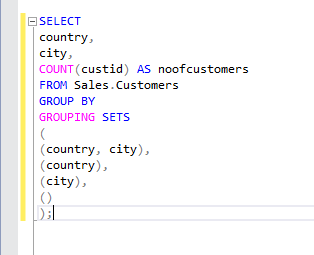
\includegraphics[width=5cm]{./Imagenes/6img1} 
	\end{center}

\textbf{}\\
Paso 4. Resalte la consulta escrita y haga clic en Ejecutar.
\begin{center}
	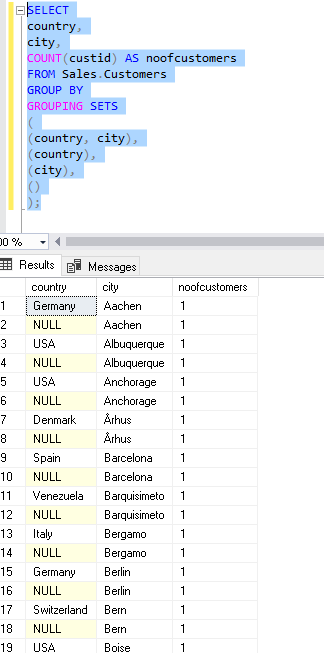
\includegraphics[width=6cm]{./Imagenes/6img2} 
	\end{center}
\textbf{}\\
\textbf{}\\


\textbf{Tarea 2: escriba una instrucción SELECT que use la subcláusula CUBE para recuperar Grupos de agrupación basados en valores de ventas anuales, mensuales y diarios.}
\textbf{}\\
\textbf{}\\
Paso 1. En el panel de consulta, escriba la siguiente consulta después de la descripción de la Tarea 2:
\begin{center}
	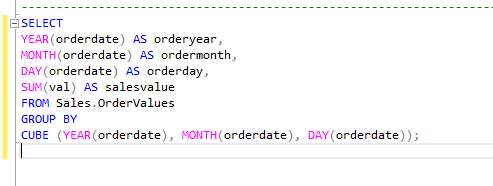
\includegraphics[width=9cm]{./Imagenes/6img3} 
	\end{center}
\textbf{}\\
\textbf{}\\

Paso 2. Resalte la consulta escrita y haga clic en Ejecutar
\begin{center}
	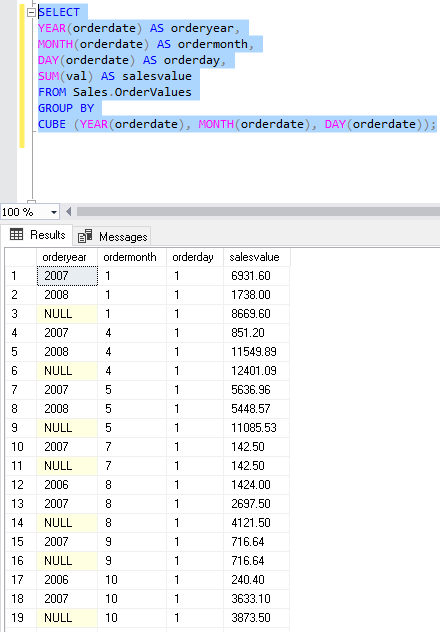
\includegraphics[width=10cm]{./Imagenes/6img4} 
	\end{center}
\textbf{}\\
\textbf{}\\


\textbf{Tarea 3: escriba la misma instrucción SELECT utilizando la subcláusula ROLLUP}
\textbf{}\\
\textbf{}\\
Paso 1. En el panel de consulta, escriba la siguiente consulta después de la descripción de la Tarea 3:
\begin{center}
	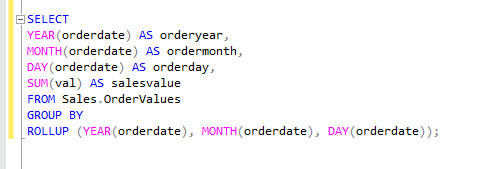
\includegraphics[width=10cm]{./Imagenes/6img5} 
	\end{center}
\textbf{}\\


Paso 2. Resalte la consulta escrita y haga clic en Ejecutar.
\begin{center}
	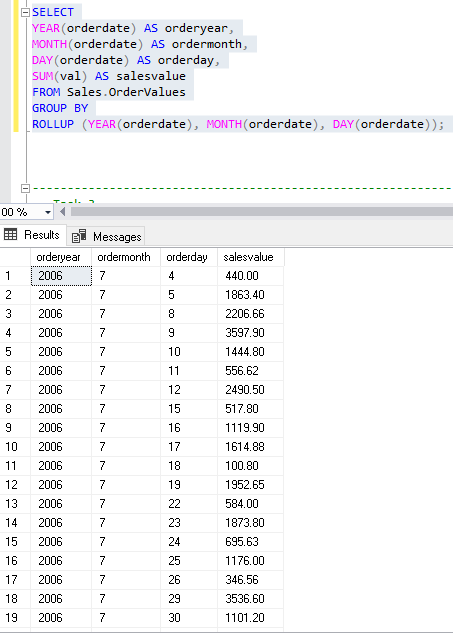
\includegraphics[width=10cm]{./Imagenes/6img6} 
	\end{center}
\textbf{}\\
\textbf{}\\
\textbf{}\\
\textbf{}\\
\textbf{}\\
Paso 3. Observa el resultado. ¿Cuál es la diferencia entre las subcláusulas ROLLUP y CUBE de la cláusula GROUP BY? 
\textbf{}\\
\textbf{}\\
Me gusta La subcláusula CUBE, la subcláusula ROLLUP proporciona una forma abreviada de definir conjuntos de agrupación múltiples. Sin embargo, a diferencia de CUBE, ROLLUP no produce todos los conjuntos de agrupación posibles que pueden definirse en función de los miembros de entrada; Produce un subconjunto de esos. ROLLUP asume una jerarquía entre los miembros de entrada y produce todos los conjuntos de agrupación. Eso tiene sentido, teniendo en cuenta la jerarquía. En otras palabras, mientras CUBE (a, b, c) produce los ocho grupos posibles de los tres miembros de entrada, ROLLUP (a, b, c) produce solo cuatro conjuntos de agrupación, asumiendo la jerarquía a> b> c.
ROLLUP (a, b, c) es el equivalente a especificar CONJUNTOS DE AGRUPACIÓN ((a, b, c), (a, b), (a), ()).
\textbf{}\\
\textbf{}\\
¿Cuál es la subcláusula más apropiada para usar en este ejemplo?
\textbf{}\\
\textbf{}\\
 Desde año, mes y día forman un Jerarquía, la cláusula ROLLUP es más adecuada. Probablemente no hay mucho interés en mostrar se acumula durante un mes independientemente del año, pero al revés es interesante.
\textbf{}\\
\textbf{}\\
\textbf{Tarea 4: Analizar el valor total de ventas por año y mes}
\textbf{}\\
\textbf{}\\
Paso 1. En el panel de consulta, escriba la siguiente consulta después de la descripción de la Tarea 4:
\begin{center}
	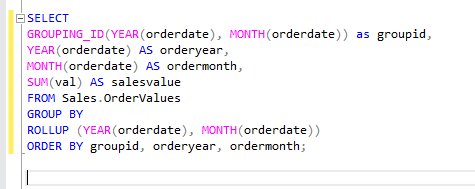
\includegraphics[width=10cm]{./Imagenes/6img7} 
	\end{center}
\textbf{}\\
\textbf{}\\
\textbf{}\\
\textbf{}\\
\textbf{}\\
\textbf{}\\

\textbf{}\\
\textbf{}\\
\textbf{}\\
\textbf{}\\
\textbf{}\\
\textbf{}\\
\textbf{}\\
Paso 2. Resalte la consulta escrita y haga clic en Ejecutar.
\begin{center}
	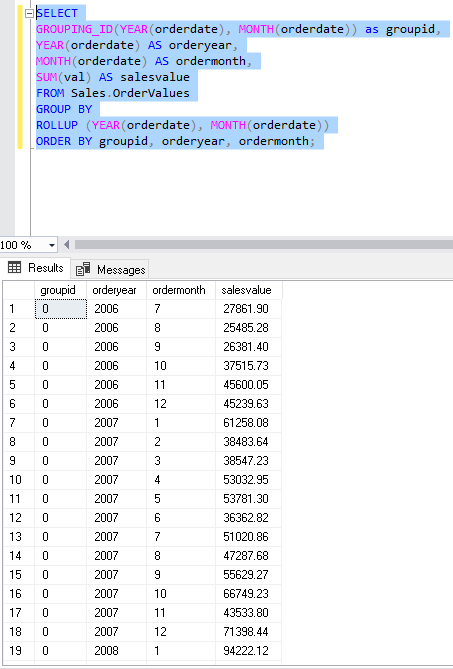
\includegraphics[width=10cm]{./Imagenes/6img8} 
	\end{center}
\textbf{}\\
\textbf{}\\








\end{flushleft}